\chapter{UML}
UML (\textbf{u}nified \textbf{m}odeling \textbf{l}anguage) è uno standard creato per unificare il modo di descrivere e progettare software in ambito della programmazione ad oggetti. 

\`E un linguaggio visuale che si basa su un meta-modello, un insieme di regole e vincoli per la modellazione di problemi software.
Ha una sintassi e una semantica ben definita. Uno dei vantaggi di UML è l'indipendenza dai linguaggi di programmazione.

I principali diagrammi trattati sono:
\begin{itemize}
\item diagrammi dei Casi d'Uso
\item diagrammi delle Classi
\item diagrammi dei Package
\item diagrammi di Sequenza
\item diagrammi di Attività
\end{itemize} 

\begin{figure}[H]
    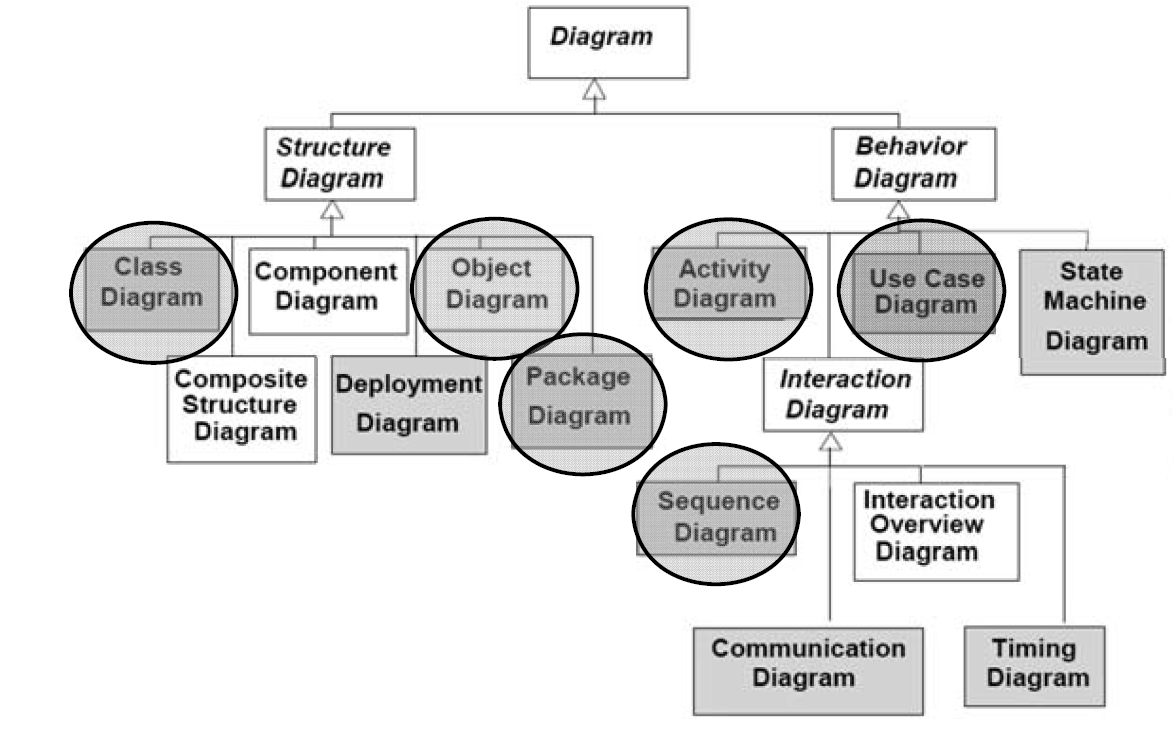
\includegraphics[width=1\textwidth]{res/img/diagrammiUML}
\end{figure}

\section{Diagrammi dei Casi d'Uso}







\section{Diagrammi delle Classi}
\section{Diagrammi dei Package}
\section{Diagrammi di Sequenza}
\section{Diagrammi di Attività}